%! TEX root = ../main.tex
\documentclass[../main]{subfiles}

% ローカル下書き用
% \documentclass{supernova_pre}
% このクラスの中に大体のパッケージは入ってるので基本何でもかけるはず
% 追加したいパッケージがあればここに記入


\begin{document}
\chapter{土星の環(リング)を考える} % タイトル
\rightline{B1 倉原ゆふ} % 学年と名前(ハンドルネームでも可)

\section{はしがき}
 2025年3月24日土星の環が消滅する,正確には"消滅して見える".これは,土星の自転軸が,公転軌道面に対して傾いていること,環の厚みが星本体と比較して非常に薄いことが原因で,地球と土星または太陽と土星が特定の位置関係にあるときに生じる.この約15年に一度のイベントにちなんで,このコーナーでは土星を中心にリングについて紹介する.
\begin{figure}[htbp]
    \centering
    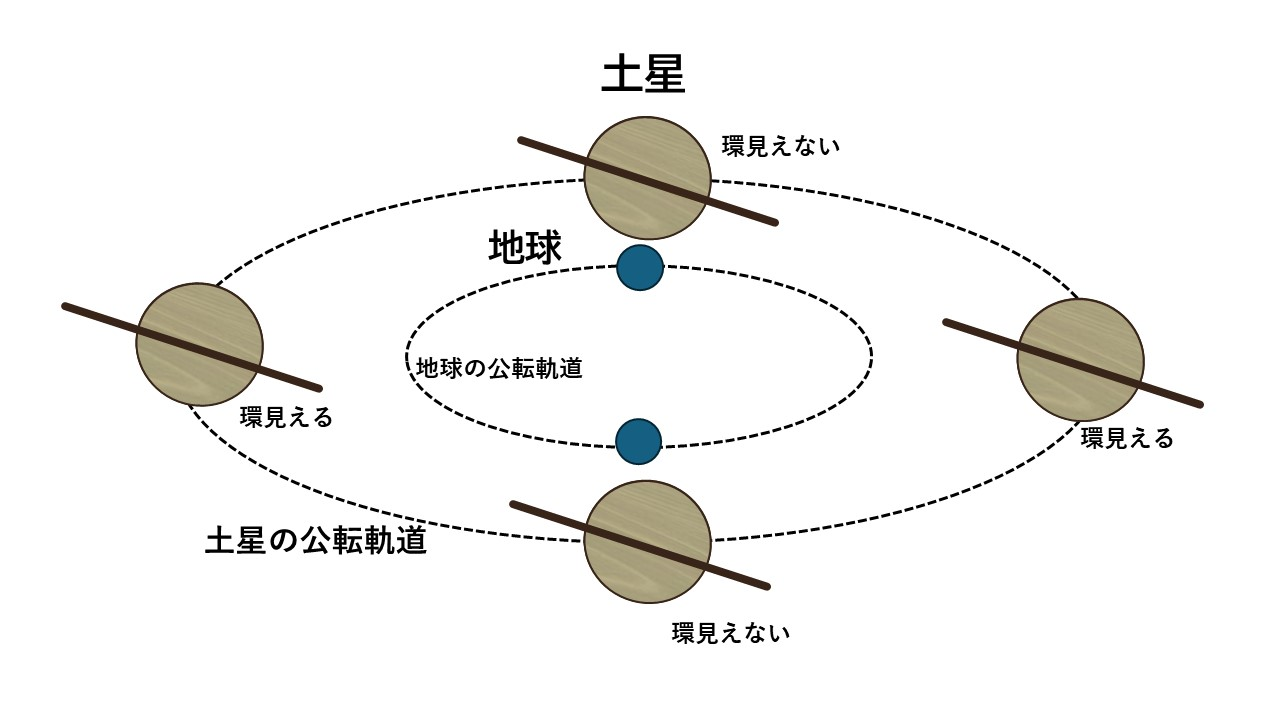
\includegraphics[width=14cm]{sections/kurahara/部誌用/スライド3.JPG}
    \caption{消失のイメージ図}
\end{figure}

\section{木星の歴史}
 1610年,ガリレオは望遠鏡によって土星に"耳"のようなものがあることを観測した.(これはテストに出る.耳を発見しただけであって,決してリングを発見したわけではないことに注意)これが人類とリングの歴史の始まりと言われている.
この後数々の研究が進み,ついに1659年,ホイヘンスによって衛星「タイタン」が発見され,これでようやく現在私たちが知るリングの姿が理解された.

\section{土星の基本データ}
 土星は巨大ガス惑星の一つである.表面は1000㎞にも及ぶ,分厚い気体水素に覆われている.その内部に液体水素層,さらにその内部に液体金属状水素層があり,鉄やケイ素塩を主成分とする核を覆っている.\\
 土星赤道付近の高層大気では$\SI[mode=text]{500}{m/s}$の風が吹き荒れている.また,北極付近には六角形にジェットが噴出している.\\
 赤道長半径は約$\SI[mode=text]{9.6}{au}$,質量は地球の95倍,自転周期は約10時間半,公転周期は約29.5年である.密度は$\SI[mode=text]{690}{kg/m^3}$と惑星の中で最小である.ちなみに水の密度は$\SI[mode=text]{997}{kg/m^3}$,地球の密度は$\SI[mode=text]{5.511E3}{kg/m^3}$であるため,天文学的なスケールだと土星の密度がいかに小さいかが分かるだろう.\\
 ほとんどの衛星は,主成分が氷である.土星の衛星は2024年2月23日現在149個見つかっており(146個という意見も)そのうち最も大きい惑星はタイタンである.\\
 土星の環の厚さは数十〜数百mである.その組成はほとんどが数㎝から数m程度の(土星本体と比較して)小さな氷の粒が集まったものからなる(G,E環はダストからなる).環は多重構造をなしており,主な土星の環は内側からD,C,B,A,F,G,E環という名前がついている.このほかにも数種類の環が発見されており,それぞれがさらに細かい環が集まって形を保っている.A,B環は,環の幅が一万キロメートルを超えるため,小さい望遠鏡でも観察可能で,その間にはカッシーニの間隙が見える.条件がよければ大きい望遠鏡を用いることで,C環も観察できるが,その他のものの観察は難しい.\\
 土星がこれほど細い環を持つ原因としては土星によって生じる重力と遠心力のつりあいが関係している.環の一点ー点では主にこの2力がはたらいており,つりあいの位置は一点に定められるからである.


\section{形成の歴史}
 土星の環の形成については諸説があるが,次の説が有力である.まず,巨大カイパーベルト天体が,土星の潮汐によって破壊されて破片が生じる.それらのうち惑星に落ち込むことなく,さらに細かい粒子となって宇宙空間に漂ったものが環を成すというものだ.\\
 カッシーニの間隙は衛星ミマスの生じる引力により存在している.ミマスは母天体の近くで運動しているため土星のロッシュ限界内にある粒子に強い共鳴作用を与えている.\\
 ここで,ロッシュ限界についてざっと説明しておく.簡単に言えば,ロッシュ限界とは重力で結合している物体の破壊条件である.ある天体から一定距離以上離れなければ,その天体から受ける力で,”重力”のみによって結合している物体は塵となってしまう(人間は化学結合によって形を成しているためばらばらにならない).土星の環はロッシュ限界内にあるため個々の重力で集まることができず,新たな天体を作ることなく粒子として宇宙空間を漂っているのだ.(まあつまり土星の環は重力とミマスの囚われの身みたいなものってことです)ロッシュ限界は天体半径の約2倍である.なお,木星は天体半径が大きすぎるがためにロッシュ限界が惑星内に位置しているため,土星のような方法で輪ができることはない.
\\\\
 さて,カッシーニの間隙について話を戻そう.ミマスの公転周期から各環の位置を見てみると,1/2周期に相当する共鳴現象によって,最も不安定な位置がカッシーニの間隙となっている.同様に,1/3周期の位置はB環の内縁に,2/3周期の位置はA環の外縁に相当する.巨視的に環構造を考える,このような原理で間隙はできている.\\
 また,これだけだとC環の密度の小ささが説明できないため,もう少し丁寧な理論が必要になる.ここで鍵となるのが密度波である.ミマスの運動が環の粒子中に疎密波を生じ,これが粒子に角運動量を与えるために間隙にある粒子にはたらく力がつり合わなくなり,環の外に逃げていくのだ.


\section{他の惑星のリング}
 あまり目立たないが木星,天王星,海王星にも環はある.これら土星のものとは異なり,主成分はダストである.\\
 木星,天王星,海王星の環は暗く,それぞれは4本,13本,4本の非常に細い環をもつ.どの環も土星と同様に,準惑星の残骸が元となっていると考えられているが,詳しい形成機構はわかっていない.

\newpage

\section{”環の消失”とは(この段落だけでも読んでくれ)}
 これからは,ついに土星消失について詳しく記述していく.\\
 土星は自転軸が公転軌道面から約26.7度傾いている.そのため公転周期の半分,すなわち約15年に一度土星の環を横から見ることができるのだ.以下に環消失のパターンをまとめた.


\begin{description}
    \item[① 地球が土星に対して横を向くとき]\mbox{}\\
     土星の赤道(=緯度0度)に地球があるときがこの時期にあたる.地球から見て土星が太陽側にある場合(”合”という),太陽が眩しすぎてあまり良い条件で観察することができない.\\
 逆に太陽と反対側にあるとき(”衝”という),環を持たない様子を非常に良く観察できるのだ.
   \begin{figure}[H]
    \centering
    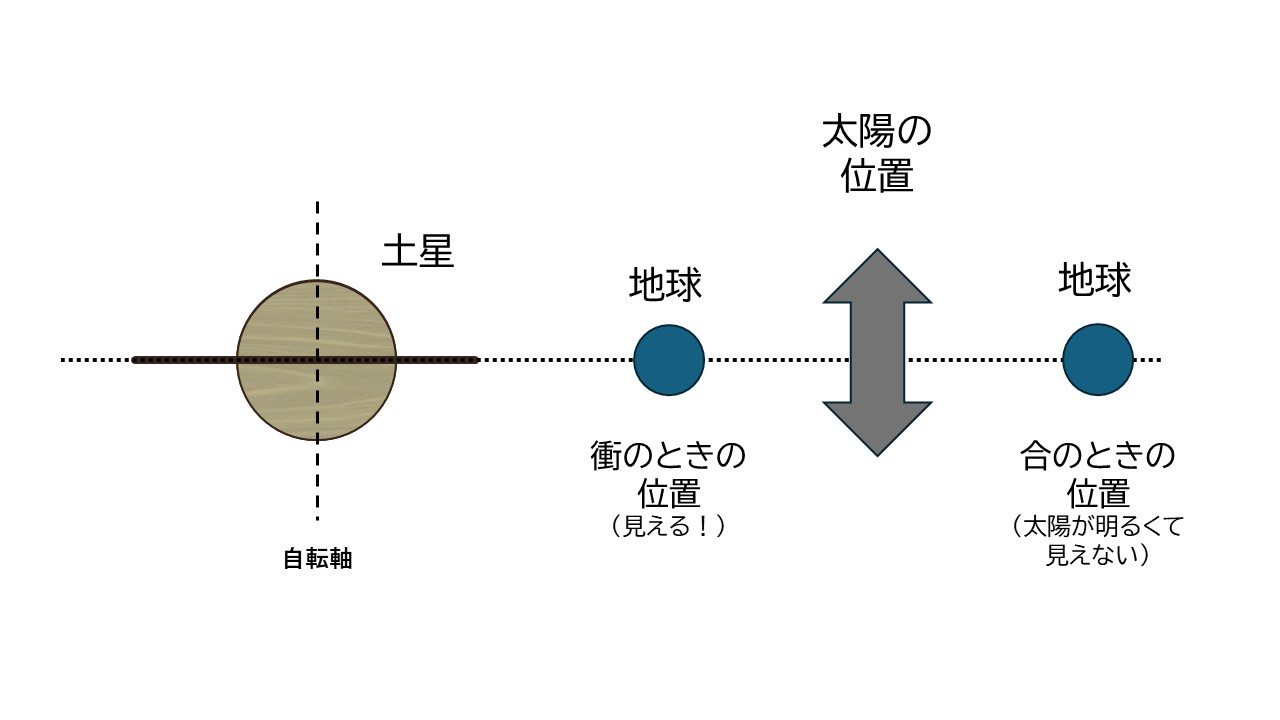
\includegraphics[width=14cm]{sections/kurahara/部誌用/スライド1.JPG}
    \caption{①のイメージ図}
\end{figure}


    \item [② 土星が太陽に対して横を向くとき]\mbox{}\\
     土星から見て赤道に太陽が来るとき(土星の春分と秋分)がこの時期にあたる.土星に対して太陽と地球は大体同じ方向にあるため,地球が土星に対して横を向くときの付近でこちらの現象も観察できる.\\
 こちらは土星の環の面に光が当たらなくなるためにほとんど見えなくなるというのが原理である.

   \begin{figure}[H]
    \centering
    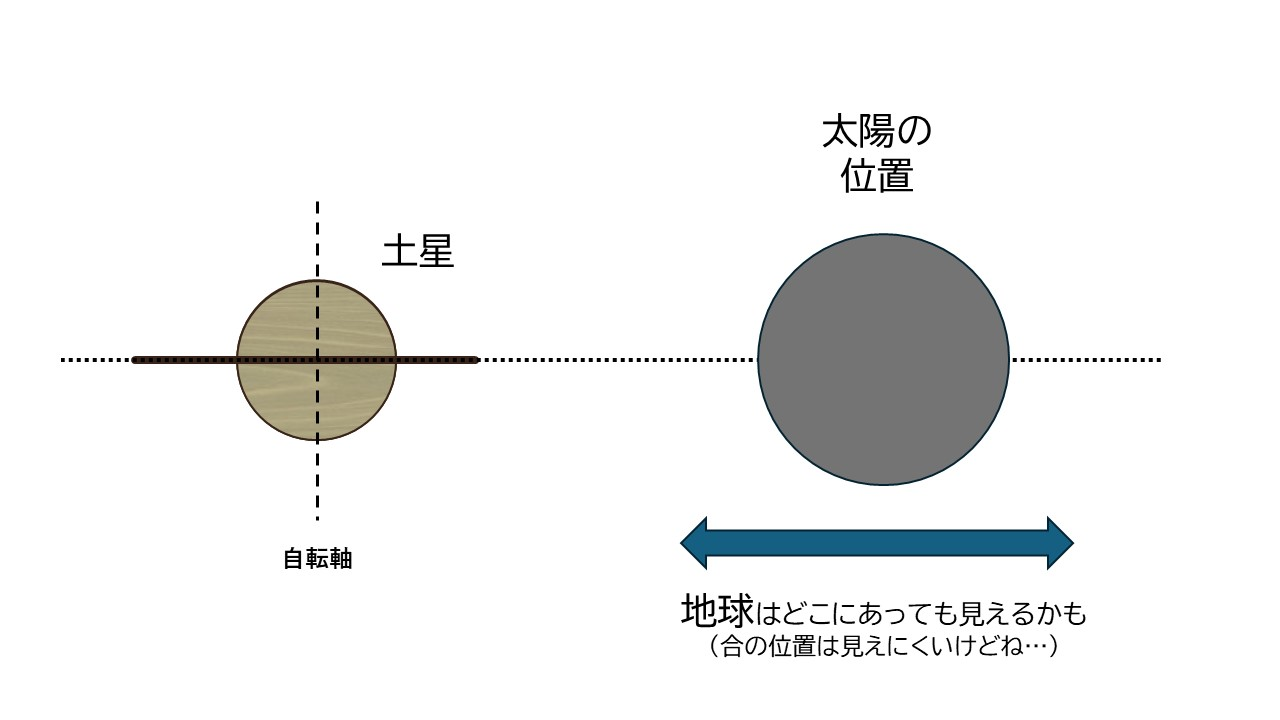
\includegraphics[width=14cm]{sections/kurahara/部誌用/スライド2.JPG}
    \caption{②のイメージ図}
\end{figure}

    \item [③ 環の陰になっているほうがみえるとき]\mbox{}\\
     太陽の光が当たっていないほうの面が見えている期間がこの時期に当たる.(①,②の間の時期)
       \begin{figure}[H]
    \centering
    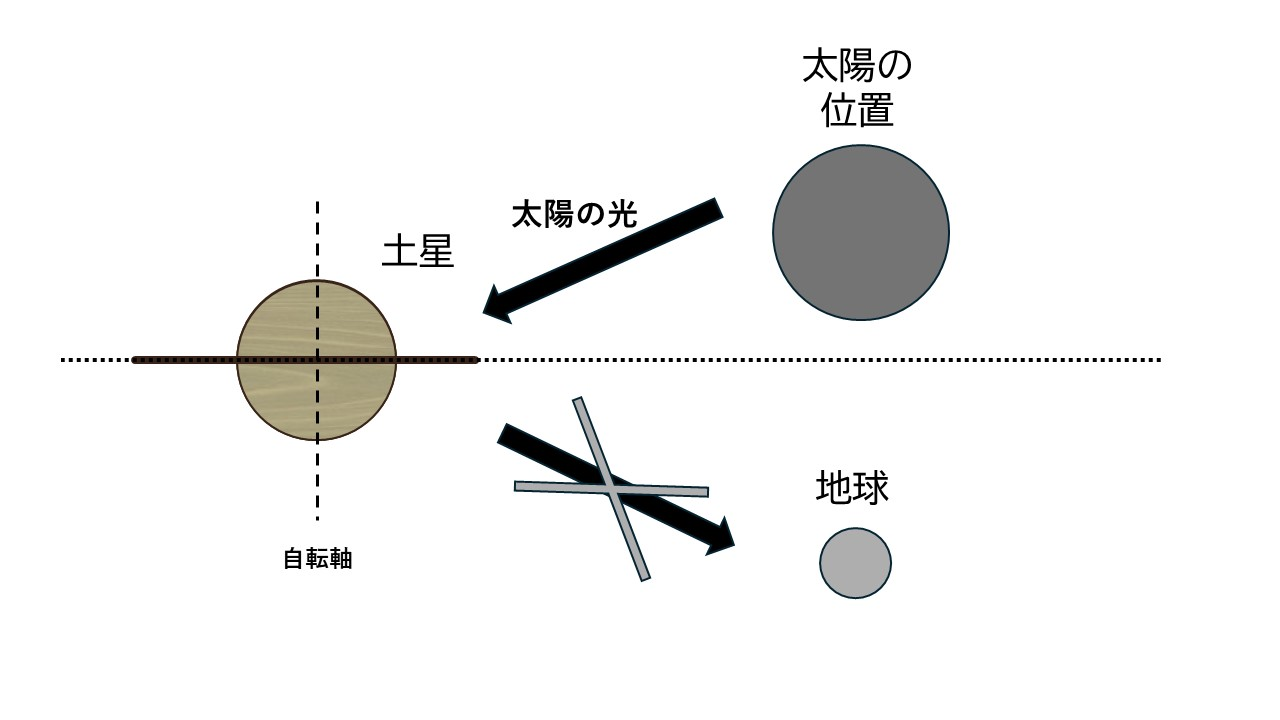
\includegraphics[width=14cm]{sections/kurahara/部誌用/スライド4.JPG}
    \caption{③のイメージ図}
\end{figure}
\end{description}


 環の消失により,環によって見えていなかった衛星を見つけやすくなったり,土星の模様がよく見えるようになったりと土星についての新たな発見が期待できる.\\
 なお,次の消失は2025年3月24日に地球が土星の北側から南側へ移り(前者の条件),続いて同年5月7日に太陽が南側へ移る(後者の条件)タイミングで見られる.ただし,3月から4月中旬までは太陽に近いため,観望には適さない.5月7日ごろは,夜明け前の東の低い空で観察できる.\\
 また,同年11月25日ごろには地球が土星の赤道方向に再び近づく.夕方から夜にかけて高度も十分にあり,観望のチャンスといえるであろう.


\section{あとがき}
 現在も徐々に環が細くなっていく様子が観察できる.皆も日々変わりゆく土星の姿を観察してみてはどうだろうか.

\begin{figure}[htbp]
    \centering
    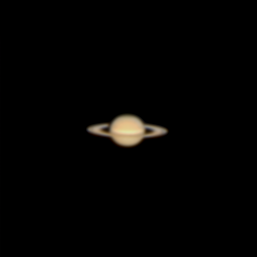
\includegraphics[width=10cm]{sections/kurahara/部誌用/retouch_stack_MVI_4355.png}
    \caption{2023年9月 撮影者:ぶちょー}
\end{figure}

\begin{thebibliography}{10}
  \bibitem{1} J.エリオット, R.カー(和訳:中村 士,相馬 充),惑星のリングはなぜあるのか,岩波書店,1987年12月18日刊行
  \bibitem{2}Star Walk,Planet Uranus: The Coldest Planet,Astronomical News,2024年10月20日更新,\url {https://starwalk.space/en/news/facts-about-uranus}
  \bibitem{3}国立天文台,惑星の衛星数・衛星一覧,2024年2月23日更新
  \newblock {\url{https://www.nao.ac.jp/new-info/satellite.html}}
  \bibitem{4}国立天文台,「土星の環の消失現象」の解説,2009年9月4日更新,\url{https://www.nao.ac.jp/phenomena/20090904/#:~:text=%E5%89%8D%E3%81%AE%E9%A0%85%E3%81%A7%E8%BF%B0%E3%81%B9,%E5%B9%B4%E3%81%94%E3%81%A8%E3%81%AB%E8%B5%B7%E3%81%93%E3%82%8A%E3%81%BE%E3%81%99%E3%80%82}
  \bibitem{5}NASA,Saturn Facts,
About the Planets,\url{https://science.nasa.gov/saturn/facts/}
\end{thebibliography}

\end{document}
